%%%%%%%%%%%%%%%%%%%%%%%%%%%%%%%%%%%%%%%%%%%%%%%%%%%%%%%%%%%%%%%%%%%%
% Eigener Ansatz
%%%%%%%%%%%%%%%%%%%%%%%%%%%%%%%%%%%%%%%%%%%%%%%%%%%%%%%%%%%%%%%%%%%%

\chapter{Konzept}
  \label{Konzept}
  
Um die Orientierung umsetzen zu können braucht man zwei Werte: Azimut und Elevation. Azimut ist die Drehung in der horizontalen und Elevation die in der vertikalen Ebene. In Euler-Winkeln gesprochen entspricht Azimut Yaw und Elevation Pitch.

\section{Accelerometer}
Das Accelerometer ist ein Beschleunigungssensor. Er misst die Beschleunigung in alle drei Richtungen. Nach unten wirkt immer die Erdbeschleunigung von $9,81ms^2$. Mit geeigneten Filter-Verfahren, wie dem Tiefpassfilter, kann man die Gravitation von der durch den Benutzer verursachten Beschleunigung isolieren. Mit dem ständig bekannten Gravitationswert ist es möglich die Lage des Geräts zu bestimmen. Jedoch sind diese Berechnungen nicht sehr genau. Das liegt zum einen an der Schwierigkeit der Trennung zwischen Gravitation und durch den Benutzer verursachten Beschleunigung und zum anderen an der Ungenauigkeit der in mobilen Geräten verbauten Sensoren. Das verursacht zusammen nach wenigen Sekunden einen so großen Fehler, dass das Accelerometer zu Berechnung der Orientierung nicht in Frage kommt.

Jedoch fließt das Accelerometer in die Gesamtberechnung trotzdem ein, denn weil das Accelerometer immer nach unten ausgerichtet ist und sich auch immer selbst wieder korrigiert, kann es zur Stabilisierung des Gyroskops verwendet werden.

\section{Gyroskop}

Das Gyroskop ist ein Drehratensensor. Es ermittelt die Winkel einer Drehung des Geräts entlang aller drei Achsen. Daraus kann sehr präzise und vor allem flüssig die Orientierung berechnet werden. Die Orientierungs-Angabe, die man aus den Gyroskop-Daten gewinnt, ist relativ zur Position des Geräts bei Beginn der Messung. Die Gyroskop-Werte von mobilen Geräten haben meist einen merkbaren Drift. Dieser hat aber den Vorteil, dass er sehr konstant ist.
  
\section{Kompass}
Der Kompass bestimmt anhand des Magnetfelds der Erde die magnetische Nordrichtung. Daraus können auch alle anderen Himmelsrichtungen bestimmt werden. Mit dem Kompass kann ausschließlich Azimut bestimmt werden. Der Kompass ist immer auf Norden ausgerichtet, er richtet sich immer wieder selbst aus. So erhält man den absoluten Azimut-Wert. Der Kompass ist anfällig auf Störungen durch jegliche Magnetfelder in seiner Umgebung. Bei mobilen Geräten stellen besonders elektromagnetische Felder, wie sie im Alltag durch viele elektrische Geräte verursacht werden, ein Problem dar. Teilweise liefert der Kompass sprunghafte Werte, die nicht für eine flüssige Darstellung der Orientierung verwendet werden können.
  
\section{Multisensordatenfusion}
Keiner der gängigen Sensoren lässt sich alleine zur Berechnung der Orientierung verwenden.

Da das Gyroskop keine absoluten Daten liefert müssen die Gyroskop-Werte, bevor man sie verwendet, einen Startwert erhalten. Auf diesen werden die weiteren Drehungen addiert. Bei Azimut nimmt man als Startwert den Kompass-Wert. Bei Elevation wird der Startwert mit Hilfe des Accelerometers berechnet. Das Accelerometer liefert auch gleichzeitig die Stabiliserung der Elevation. So kann der Drift des Gyroskops zuverlässig vermieden werden. Bei Azimut wird der Kompass als Startwert-Geber herangezogen. Zur Stabilisierung fließt der Wert des Kompasses leicht in den Gyroskop-Wert ein. Dies geschieht mit folgender Formel:

$$f(\alpha, \phi) = (\alpha*updatedHeading +\phi*heading)/(\alpha+\phi)$$\label{formula001}

Wobei $heading$ der jeweils neue Kompass-Wert ist und $updatedHeading$ der alte Azimut-Wert auf den die Drehung, ermittelt durch das Gyroskop, addiert wurde. $\alpha$ und $\phi$ sind die Gewichtungen von $heading$ und $updatedHeading$. Schaubild \ref{fig:struktur} ist eine visuelle Darstellung dieser Vorgehensweise.
 

\begin{figure}[htb]
\centering
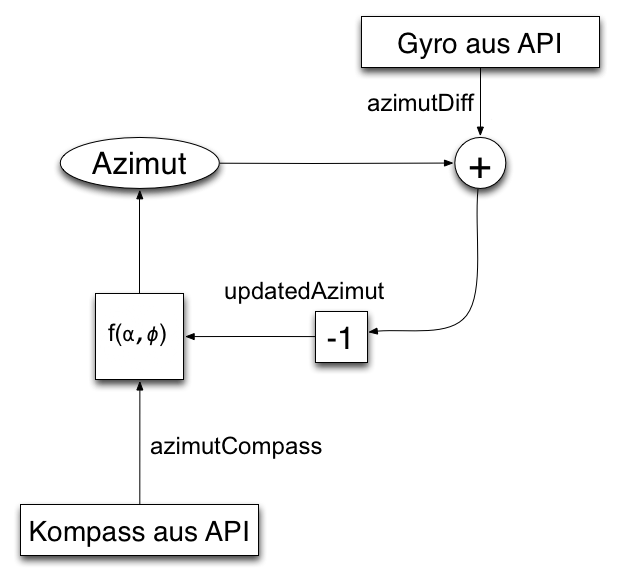
\includegraphics[scale=0.5]{figures/struktur}
\caption{Konzept Multisensordatenfusion}
\label{fig:struktur}
\end{figure}






